%\documentclass[draftclsnofoot,onecolumn]{IEEEtran}
\documentclass[3p]{elsarticle}
\usepackage{tipa}
\usepackage{amsmath}%math
\usepackage{amsthm}%proof
\usepackage{xcolor}%color
\usepackage{bm}
\usepackage{graphicx}
\usepackage{booktabs}
\usepackage{textcomp}
\usepackage[colorlinks,linkcolor=black,anchorcolor=black,citecolor=black]{hyperref}
\usepackage{amsfonts,amssymb}
\usepackage{color,soul}
\theoremstyle{plain}
\newtheorem{assumption}{Assumption}
\newtheorem{mydef}{Definition}
\newtheorem{mylem}{Lemma}
\newtheorem{myrem}{Remark}
\newtheorem{thm}{Theorem}
\begin{document}
\begin{frontmatter}
\title{Adaptive Sliding Mode Control of Tethered Satellite  Deployment with Input Limitation}
\author{Zhiqiang Ma}
\author{Guanghui Sun\corref{cor1}}
\ead{guanghuisun@hit.edu.cn}
\cortext[cor1]{Corresponding author}
\address{Research Institute of Intelligent Control and Systems, Harbin Institute of Technology, Harbin 150001, China}

\begin{abstract}
This paper proposes  a  novel adaptive sliding mode tension control method for  the deployment of tethered satellite, where the input tension limitation is taken into account. The underactuated governing equation of the tethered satellites system are firstly derived based on Lagrangian mechanics theory. Considering the fact that the tether can only resist axial stretching, the tension input is modeled as input limitation. New adaptive sliding mode laws are addressed to guarantee the stability of the tethered satellite deployment with input disturbance, meanwhile to eliminate the effect of the limitation features of the tension input. Compared with the classic control strategy, the newly proposed adaptive sliding mode control law can deploy the satellite with smaller overshoot of the in-plane angle and implement the tension control reasonably and effectively in engineering practice. The numerical results validate the effectiveness of the proposed methods.
\end{abstract}
\begin{keyword}
Tethered satellite;  Adaptive control;  Sliding mode;  Input limitation
\end{keyword}
\end{frontmatter}
\section{Introduction}
\textcolor{red}{The system of satellites connected by space tethers is a kind of artificial objects in space and was proposed by Guiseppe Colombo and Mario Grossi in 1960s. Since then, more than twenty orbital and suborbital experiments have been implemented by many institutes,} such as TSS-1R \cite{lanoix2005effect}, SEDS, MAST, YES2 \cite{williams2012review} and so on.
\textcolor{red}{The tethered satellite system (TSS) is applied widely in scientific tasks}, such as energy collection with the tether (wire) shuttling in the magnetic field of the Earth \cite{lanoix2005effect}, deorbit of the subsatellite \cite{khan2014analysis}, space tug \cite{wen2016constrained} and space elevator \cite{kojima2015mission}. The TSS is expected to be competent for works like rescuing stranded astronauts, capturing target capsules \cite{huang2015adaptive}, satellite formation flights \cite{hallaj2015tethered,alary2015dynamics}, establishing the artificial gravity field, providing the micro gravity experiment environment \cite{chung2007nonlinear} and so on.\par
The deployment/retrival mission of tethers is interesting and delicate to be studied on \cite{Fujii2012Deployment,steindl2014optimal,cai2014deployment,ma2014coordinated,jung2015nonlinear,li2016libration}.
\textcolor{red}{In the past decade, some groups came up with some research achievements in regulating the deployment/retrival of the TSS.}
All of these techniques can be divided into two types, the tension approach with thrusters and the pure tension approach, respectively. The thruster strategies focus on employing thrusters to fix the out-of-plane angle.
For example, Liu considered the model with the equipped thrusters fixing the out-of-plane angle, and proposed the variable structure scheme to complete the mission of the deployment \cite{yingying2012variable}. Furthermore, during the mission, the thrusters were also applied to make the acceleration of the tether persist so that the tension sustains positive at the same time. Huang presented a robust adaptive backstepping method to achieve stabilization of a tethered space robot-target combination, and the thrusters were assumed to provide the constant control torque during the mission \cite{huang2015adaptive}. Owing to the high complexity and consumptions in equipment of the thrusters, it's a challenge to implement thruster approaches to regulating the dynamics of the deployment/retrieval in practice. Therefore, more and more researchers make efforts to investigate different tension control strategies, such as analytical feedback control law \cite{wen2015space}, nonlinear dynamic methods \cite{jung2015nonlinear}, LQG \cite{yousefian2015anti}, optimal control strategies \cite{steindl2015optimal,Williams2009745} and so on. The number of existing control schemes is larger than the utilized one in practice with respect to strict physical constraints, such as the limited output of a tension actuator and the restrained mechanics characteristics of tethers. Zhu proposed a law in an analytical feedback form to achieve the stability of the motions of the tethered space-tug system during its deorbiting process, and in the scheme two specializing saturation terms were applied to maintain the tension positive \cite{wen2016constrained}. \textcolor{red}{Moreover, considering the physical restriction including the bounded tension and the underactuated characteristics in practice engineering,} the variable structure control methods have also been studied in the field of the motion regulation of the TSS. A sliding mode control approach was developed to complete the mission of the deployment and the retrieval by using substellite jets. In the mission, the tether direction was directly controllable with the thruster system which was equipped on the subsatellite and generated the control torque to regulate the motion of the tethered system, and with the help of the thrusters, the tension that acts on the tether was always kept positive \cite{yingying2012variable}.
Specifically, the input in the presented sliding mode controller was provided by the in-plane and out-of-plane thrusters, hence, the limitation of the tension was avoided, as the tether length rate remained constant. Soon-Jo introduced the nonlinear model reduction techniques of the tethered formation flight and mentioned the sliding mode control scheme for the stability of the TSS \cite{chung2007nonlinear,chung2008propellant2}. However, in the mention above control design for the attitude regulation, the characteristics of the coupled input in the underactuated mode was studied particularly, but the analysis about the issue of the tether tension was not present, as the tether length in the model was designed as a constant value.\par
It's noteworthy that above mentioned schemes or laws don't concentrate on issues about the limitation of the input and the underactuated characteristics especially. In perspective of the controller design, the limitation of the input has not been considered into the synthesis of control strategies, whereas thrusters or jets, as the source of the system input, are equipped on subsatellites to handle the underactuated dynamics. The thruster augmentation which has been recommended by Banerjee and Kane increases both the mass and the power requirements of the TSS \cite{banerjee1984tethered}, whereas the deployer driven by using a reel mechanism can control the speed of the deployment more simply and directly. There is one point which needs attention that the space span of the TSS is larger than other artificial celestial ones relatively, and it's necessary to consider tensile properties of the tether in the complex space environment. From the standpoint of practical applications, the break of the tether leads to the failure of the deployment mission as the result of the tension over the tolerance, and moreover, the compression will not happen to the tether. Hence, considering the pure tension control, the output of the tension actuator is limited during the deployment mission.\par
In this paper, an adaptive sliding mode control scheme is proposed for regulating the length of the tether and the in-plane angle of the TSS during the deployment. Specifically, the thruster doesn't attended for steering the pitch or roll angle so that the system becomes underactuated, and in this case only the dynamics of the in-plane deployment is paid attention to. To cope with the limitation of the tension actuator, an innovative adaptive update rate is given to assure that the variable structure control system is stable with Lyapunov stability theory. For the isolated in-plane plant, based on the variable structure control theory, a discontinuous control scheme is derived to accomplish the deployment with the uncertainties and the external disturbance. The proposed adaptive sliding mode control scheme guarantees the global reaching condition in a rapid convergent speed.\par
The paper is organised as follows. Section \ref{sec:mm} puts forward the rigid model of the TSS in the deployment mission based on Lagrangian mechanics theory. The state feedback adaptive sliding mode control scheme with the input limitation is illustrated by utilizing Lyapunov stability theory in Section \ref{sec:SMC}, and the finite-time convergence property is explained there. In Section \ref{sec:sm}, for validating the techniques mentioned, the mission example of the deployment is implemented, and the associated simulation results demonstrate that the control schemes presented in this paper are effective and robust. Conclusions are given in Section \ref{sec:Conclusion} finally.
\section{Mathematical modelling}\label{sec:mm}
The TSS is idealized as a simplified problem of the rigid model shown in Figure~\ref{fig:model}, and the description of the coordinate system is given firstly.
\begin{figure}
\centering
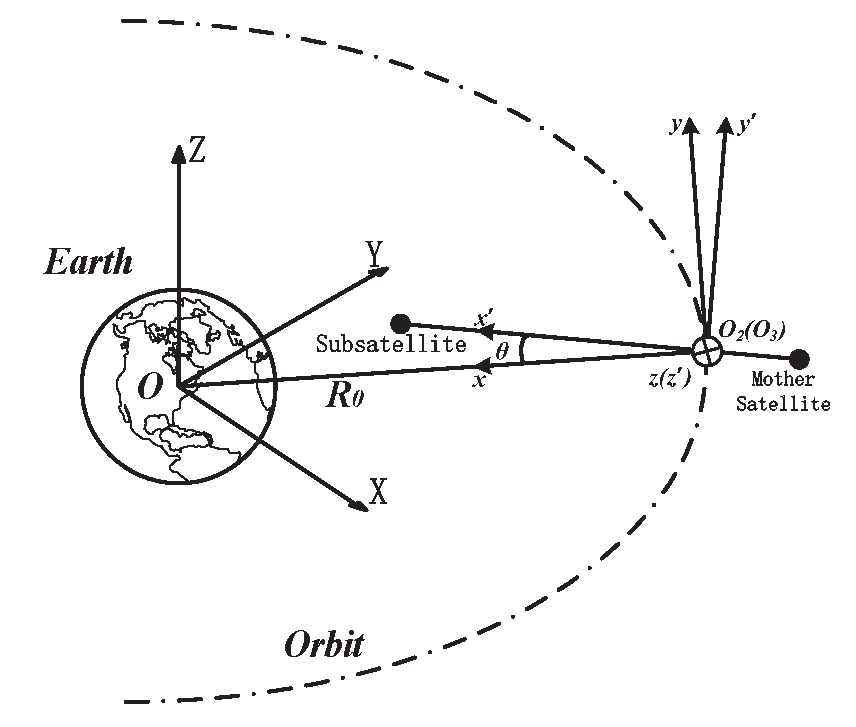
\includegraphics[width=6.94cm,height=5.87cm]{orbit_in_plane.eps}
\caption{Tethered satellite system rigid model}\label{fig:model}
\end{figure}
Define $OXYZ$ as the inertial frame, whose origin $O$ is located at the center's core, and $OX$ points towards the spring equinox on the equatorial plane; $OZ$ bundles the earth's rotation axis upwards; $OY$ is generated with the right-hand rule.
Define $O_2xyz$ as the orbital coordinate system, and the origin $O_2$ denotes the centroid of the tether system. $O_2y$ is heading of the orbital, and $O_2x$ means the direction to the earth downwards. $O_2z$ is generated with the right-hand rule, and in addition, $\theta$ expresses the tether in-plane libration angle. In fact, the out-of-plane behavior is coupled with the length of the tether, however, the performance of the in-plane angle and the  out-of-plane angle can not be compatible without thrusters fixing the out-of-plane dynamics\cite{Vadali1991Feedback}. On the other hand, the excursion of the out-of-plane angle is not big, when the in-plane behavior is controlled stably, the out-of-plane one is steady incidentally in the condition that the initial out-of-plane libration angle and the angular rate are approximately both $0$ rad. \textcolor{red}{Based on the above analysis, the out-of-plane behavior has practically no influence to the dynamics of the deployment. Hence the analysis of the out-of-plane behavior is omitted here, and in this work, the dynamics of the in-plane deployment is paid attention to primarily. Define $O_3x'y'z'$ as the tether system frame, and $O_3x'$ points to the subsatellite along the tether. It's assumed that the axis $O_3z'$ is fixed to axis $O_2z$ for the in-plane deployment is investigated only in this work. Hence, the in-plane tether system frame $O_3x'y'$ can be obtained by rotating $O_2xy$ along the fixed axis $O_3z'$ ($O_2z$), and $O_3$, $O_2$ are always coincident. $\bm{R}$ and $\bm{r}$ represent the position vector of the system in relation to $O,O_2$, respectively. $\bm{R_0}$ denotes the position vector of $O_2$ in relation to $O$.}\par
For the deployment of the TSS, most of the control schemes give a basic assumption that the motion can approximate to a ``rolling ball'' behavior and can be modeled with three DOFs. It's reasonable to establish a model with the spherical coordinates describing the behavior of the satellites. The mass of the tether can be ignored sufficiently, because it's far less than the mass of the mother satellite. Some other critical assumptions throughout the analysis of modeling are outline next. The satellites are treated as particles provided that the length of the tether is far larger than the size of the satellites. The ratio of the mass between the subsatellite and the mother satellite is tiny so that the mother satellite can stay in its nominal orbit, and the action of the subsatellite doesn't make the attitude of the mother satellite out of the control. The system is forced by the gravitational force of the Earth and the tension acting on the tether. Besides that, it's reasonable to regard the tether as inextensible, straight and massless in modeling, and the tether can stay stiff and taut during the libration.\par
Before modeling the system, some preliminary important symbols are given to avoid the possible misunderstanding, the radius of orbit without disturbance, $R_0$, the orbital angular velocity, $\Omega=\sqrt{\mu_e/R_0^3}$, the coefficient of the Earth gravity field, $\mu_e$. \par
Using the assumption of the circular orbit, based on Lagrangian mechanics theory, the kinetic energy and the potential energy of the TSS can be expressed as follows respectively
\begin{align}
T_t
&= \frac{1}{2}\sum\limits_{s=1}^2 m_s\bm{R_s'\cdot R_s'}\notag\\
&= \frac{1}{2}m\bm{R_0'\cdot R_0'}+\frac{1}{2}\sum\limits_{s=1}^2 m_s\bm{r_s'\cdot r_s'}\notag\\
&= \frac{1}{2}m\Omega^2R_0^2+\frac{1}{2}\bar{m}l^2(\theta'+\Omega)^2+\frac{1}{2}\bar{m}l'^2\label{eq:Tt1}\\
V_g
&= -\mu_e\sum\limits_{s=1}^2\frac{m_s}{\vert \bm{R_0+r_s}\vert}\notag\\
&= -m\Omega^2R_0^2+\frac{\bar{m}\Omega^2l^2}{2}(1-3cos{^2\theta})\label{eq:Vg}
\end{align}
\textcolor{red}{where, the masses of mother satellite and subsatellite are denoted as $m_1$ and $m_2$, respectively, thus the total mass of the system is symbolized by $m=m_1+m_2$}. $()'$ represents the differentiation of $()$, and $l$ is the length of the tether connecting the subsatellite to the mother satellite. $\theta$ is the in-plane angle that may describe the rolling dynamics of the TSS. For simplifying the expression of the formula, $\bar{m}$ denotes $m_1m_2/m$. $v_e$ is the argument of latitude, and $\Omega = v_e'$ may be determined with the assumption that the orbit is circular.\par
Combining Eq.(\ref{eq:Tt1}) and Eq.(\ref{eq:Vg}), let $L =T_t-V_g$, and ${q}=(\theta,l)$ denotes the generalized coordinate vector. By utilizing Lagrangian mechanics theory, the dynamic equations for the system may be obtained \cite{Williams2009745}
\begin{align}
\begin{split}
&\theta''+2(\theta'+\Omega)l'/l+3\Omega^2sin{\theta} cos{\theta}=Q_\theta/(\bar{m}l^2)\\
&\l''-l[(\theta'+\Omega)^2+\Omega^2(3cos{^2\theta}-1)]= -\tau/\bar{m}\label{eq:motion1}
\end{split}
\end{align}
where \textcolor{red}{$\tau$ is the tether tension}, and the generalized force $Q_\theta$ is related to $\theta$. In a pure tension control law design, the tension which acts in the in-plane deployment is unique for the system, thus $Q_\theta$ is typically approximate to zero. There is a critical implicit essential condition $0<\tau_{min}\le \tau\le \tau_{max} < \infty$, that the existence of $\tau_{max}$ prevents the invalid tension from tearing the tether. $\tau_{min}>0$ guarantees that the tension is positive, because the tether should be kept taut and can not be compressed during the deployment \cite{williams2008deployment}.\par
For simple expression, introduce the dimensionless conversion
\begin{align}
\begin{split}
&\lambda=l/L\\
&d()/dt=\Omega d()/dv\\
&\hat{\tau}=\tau/(\bar{m}\Omega^2L)\label{eq:varcon}
\end{split}
\end{align}\par
Note that the dimensionless tether length, $0<\lambda \le 1$, the orbit true anomaly, $v$ and the dimensionless tension, $\hat{\tau}$. $L$ is the total length of the tether. The above system is singular before the beginning of the deployment, and as a result, the dimensionless tether length is positive from the beginning of the deployment.\par
Substitute Eq.(\ref{eq:varcon}) into Eq.(\ref{eq:motion1}), then the equations are transformed into the dimensionless form under a reasonable assumption that the orbit stays unperturbed, for the reason that the time spans of deployment is too tiny to be considered in the total mission and the mother satellite is much bigger than the satellite and tether's.
Since the tether can be librated to any desired position from an available initial one, that won't cause the singular situation, there exists a variable conversion $\xi =\lambda - a$, where $a\in(0,1]$ represents the desired length of the tether. If $a=0$ is satisfied, the deployment dynamics become a singular system.\par
Set the state vector $\bm{x} = (\xi,\dot\xi,\theta,\dot\theta)^T$, then the dynamic equations of the deployment system structure can be derived into the expression by using the state space model technique under the assumption of a Keplerian reference orbit for the centroid.
\begin{align}
\begin{split}
\dot{x}_1&=x_2\\
\dot{x}_2&=(a+x_1)[(x_4+1)^2-1+3cos{^2x_3}]-\hat{\tau}\\
\dot{x}_3&=x_4\\
\dot{x}_4&=-2\frac{x_2}{x_1+a}(1+x_4)-3cos{x_3}sin{x_3}\label{eq:state}
\end{split}
\end{align}\par
The deployment mission spends the time $\delta$, thus the performance of the control system should be $t\in [t_0,t_0+\delta],t\to t_0+\delta,x_1\to 0,x_3\to x_{3d}$. According to the analysis for the TSS, the equilibrium point of the system is arbitrary. In this case the approximate linearization techniques may be implemented, and the equilibrium point can be selected as $\xi = 0$, $\dot\xi = 0$, $\theta = 0$ and $\dot\theta = 0$. Hence, the linearization expression is presented:
\begin{align}
\dot x(t) &= Ax(t) + Bf_{b}(u(t)) + \tau_d\label{eq:ABC}
\end{align}
\textcolor{red}{where $A\in R^{4\times4}$ is the system matrix which can be obtained by using Jacobian linearization method:
\begin{align}
A=\begin{bmatrix}
0 &1 &0 &0\\
3 &0 &0 &2a\\
0 &0 &0 &1\\
0 &-2/a &-3 &0
\end{bmatrix}
\end{align}}\\
and $B$ is the $4\times1$ input matrix which can be written as $[0,1,0,0]^T$  directly. Notice the second equation of Eq.(\ref{eq:state}) after applying Jacobian linearization method to it, and the input term turns to $3a-\hat{\tau}$. Symptom $u(t)$ denotes the input term which is generated by program and is actually limited as well as the generalized tension, and once the program command is over the boundary of the tension actuator's output, the limitation phenomenon emerges to lead that the input $u(t)$ is truncated. Considering the properties of the bounded tension $0<\tau_{min}\le \tau\le \tau_{max} < \infty$, the mathematics expression follows
\begin{equation}
f_b(u(t)) =\begin{cases}
3a-\hat{\tau}_{min}   & u(t) > 3a-\hat{\tau}_{min}\\
u(t)           & 3a - \hat{\tau}_{max} \le u(t) \le 3a-\hat{\tau}_{min}\\
3a-\hat{\tau}_{max}   & u(t) < 3a - \hat{\tau}_{max}
\end{cases}\label{eq:f_b}
\end{equation}
where $\hat{\tau}_{min} = \tau_{min}/(\bar{m}\Omega^2L)$ and $\hat{\tau}_{max} = \tau_{max}/(\bar{m}\Omega^2L)$. The upper limit of the tension $\tau_{max} $ is related to the tension tolerance, the orbit altitude and the deployment distance, and exact numerical results will be given in Section \ref{sec:sm}. $\tau_{min}$ exists to guarantee that the tether is taut during the deployment. It's essential to tell a result $\hat\tau_{min}<3a<\hat\tau_{max}$ which is a related condition for the design of the adaptive controller. In addition to this, note that the limitation expression hasn't to be symmetrical strictly, \textcolor{red}{and the property of the limitation is going to be discussed in next section.} \textcolor{red}{$\tau_d$ denotes the interference torque such as gravity gradient torque, solar radiation pressure torque, aerodynamic torque and magnetic torque. Thanks to previous researches, in the low orbit altitude the solar radiation pressure torque and the aerodynamic torque are both approximate to $1\times 10^{-5}$ Nm; the gradient torque is around the value range of $1\times 10^{-5}$ Nm. Without loss of generality, the perturbation term is treated as a periodic function in this work, the period of which is 5000 s approximately equaling the orbital period \cite{liu2013calculation,inamori2015magnetic}. based on the above conditions, for verifying the effectiveness of the control scheme, the tension actuator is thought to be disturbed by a sinusoidal perturbation whose amplitude is no more than $5\times 10^{-2}$ Nm with $2\times 10^{-4}$ Hz of the frequency, which represents the mentioned environment disturbance satisfying the following matching condition:
\begin{equation}
\tau_d=Bg(x,t)
\end{equation}
where $g(x,t) = 0.05\sin(2\pi t /5000)$. Hence the specific form of the disturbance can be described by
\begin{align}
\tau_d = [0,0.05\sin (2\pi t /5000),0,0]^T\label{eq:disturbance}
\end{align}}\par
In this work, we focus on the statement of Eq.(\ref{eq:ABC}) and design a nonlinear controller with the input limitation such that $\theta$ and $\lambda$ can be manoeuvered in the in-plane system as desired.
\section{Description of sliding mode control system}\label{sec:SMC}
The variable structure control system has several unique features such as rapid response, corresponding parameters and disturbance insensitive, and simple physical realization. However, considering the system with input limitations, there also exists an obstacle that conventional synthesis strategies don't take the input limitation into consideration, thus the performance of systems can not be guaranteed when the limitation occurs \cite{Hu2008Robust}.\par
Consider the dynamic equations of the in-plane deployment shown in system (\ref{eq:ABC}) with the input limitation, and the limited input $f_{b}(u(t))$ can be expressed as
\begin{equation}
f_b(u)=R(u(t))u(t)\label{eq:satu}
\end{equation}\par
Note that $0 < R(u) \le 1$
\begin{equation}
R(u) =\begin{cases}
u_{max}/u   & u > u_{max}\\
1           & u_{min} \le u \le u_{max}\\
u_{min}/u   & u < u_{min}
\end{cases}\label{eq:ru}
\end{equation}
where $u_{max}$ and $u_{min}$ are the input boundaries representing the boundaries of the output of the actuator in practice, and there exists a restriction that $u_{min}<0<u_{max}$ for guaranteeing the characteristics in the above expression: $0<R(u)\le 1$. \par
Throughout this paper, the following remark includes some crucial meaningful assumptions and essential conditions for the design of the adaptive sliding mode controller.
\begin{myrem}
\textcolor{red}{As stated in \cite{Hu2008Robust}, there exist two meaningful assumptions that can be referenced in this work.} The first one is the assumption of the controllability of the system, and the other one is the format assumption of the input disturbance. Combining the assumptions and the practice conditions yields the following characteristics of the deployment dynamics.\par
The dynamic equations of the deployment can be expressed as Eq.(\ref{eq:ABC}), without considering the input limitation, \textcolor{red}{and the triplet $(A,B)$ of the nominal system is controllable according to the rank criterion.} However, the tension acting in the TSS is strictly bounded in practice so that the conventional control strategies will fail in the regulation of the deployment. Hence, an effective control law for regulating the deployment with the input limitation is desperately needed.\par
For the external distance, $\tau_d$ is the uncertain part of system (\ref{eq:ABC}), and satisfies the following matching condition:
\begin{equation}
\tau_d=Bg(x,t)
\end{equation}
where $g(x,t) = 0.05\sin(2\pi t /5000)$, and $||g(x,t)||\le \alpha$ where $\alpha$ can be decided conveniently.
\label{as:1}
\end{myrem}
In the next section, the design process of an adaptive state feedback sliding mode controller is derived, and the controller is proposed to guarantee the stability of the deployment dynamics.
\subsection{SMC design with input limitation}
Apply the following state transformation to simplify the control design procedure
\begin{equation}
\bar{x}(t) = Tx(t)\label{eq:Tx}
\end{equation}
where $T=\begin{bmatrix}O_{2\times 2} &I_{2\times 2}\\ I_{2\times 2} &O_{2\times 2}\end{bmatrix}$ is the transformation matrix to let
\begin{equation}
TB =
\begin{bmatrix}
T_1\\T_2
\end{bmatrix}B
=
\begin{bmatrix}
O_{3 \times 1}\\B_1
\end{bmatrix}\label{eq:TB}
\end{equation}
where $T_1 \in R^{3\times 4}$, $T_2 \in R^{1 \times 4}$ and $B_1 \in R$ is nonsingular. Since $B$ has full rank, the transformation always exists. Reform the system matrix by utilizing the transformation Eq.(\ref{eq:Tx}), and yields
\begin{equation}
\dot{\bar{x}} = \bar{A}\bar{x}(t) + \bar{B} g(T^{-1}\bar{x},t) + \bar{B} f_b(u(t)) \label{eq:barABC}
\end{equation}
where
\begin{align*}
\bar{A} &= TAT^{-1}=\begin{bmatrix}
A_{11_{3\times 3}}
&A_{12_{3\times 1}}\\
A_{21_{1\times 3}}
&A_{22_{1\times 1}}\end{bmatrix}\\
\bar{B} &= TB = \begin{bmatrix}O_{3\times 1}\\B_{1}\end{bmatrix}
\end{align*}\par
The desired sliding mode surface of the proposed control system can be designed as
\begin{equation}
S(t) = \bar{C}\bar{x}(t)\label{eq:S}
\end{equation}
in which $\bar{C} = [\bar{c}_1,\bar{c}_2]\in R^{1\times 4}$ is the constant vector, and $\bar{c}_1\in R^{1\times 3},\bar{c}_1\in R$. $\bar{C}$ can be decided by the techniques deployed in article \cite{lyshevski2012control}.\par
Rewrite Eq.(\ref{eq:S}) as
\begin{equation}
S(t) = \bar{c}_1\bar{x}_1(t)+\bar{c}_2\bar{x}_2(t)
\end{equation}
\textcolor{red}{where $\bar{x}_1 =(\theta,\dot \theta,\xi)^T\in R^{3\times 1}$, $\bar{x}_2 = \dot \xi\in R$ and $\bar{x} = [\bar{x}_1^T \quad \bar{x}_2]^T$, therefore $\bar{x}_2$ follows}
\begin{equation}
\bar{x}_2(t) = \bar{c}_2^{-1}(-\bar{c}_1\bar{x}_1(t)+S(t))\label{eq:barx2}
\end{equation}\par
Substitute Eq.(\ref{eq:barx2}) into Eq.(\ref{eq:barABC}), and it follows that
\begin{align}
\dot{\bar{x}}_1(t) &= (\bar{A}_{11}-\bar{A}_{12}\bar{c}_2^{-1}\bar{c}_1)\bar{x}_1(t)+\bar{A}_{12}c_2^{-1}S(t)\label{eq:barx1}\\
\dot{\bar{x}}_2(t) &= (\bar{A}_{21}-\bar{A}_{22}\bar{c}_2^{-1}\bar{c}_1)\bar{x}_1(t)+\bar{A}_{22}c_2^{-1}S(t)\notag\\&+B_1f_b(u(t))+B_1g(T^{-1}\bar{x},t)
\end{align}
in which the behavior of system (\ref{eq:barABC}) in the desired sliding mode surface is governed by Eq.(\ref{eq:barx1}). $\bar{c}_2$ is invertible, and conditions given in \cite{lyshevski2012control} guarantee that the prescribed non-zero and complex eigenvalues $\{\lambda_1,\lambda_2,\lambda_{3}\}$ with $Re(\lambda_i)<0,i=1,2,3$, can be assigned.
After decision of the sliding mode surface, an adaptive control input is needed to be chosen so that the trajectories of the states of system (\ref{eq:barABC}) are driven onto the designed sliding mode surface in finite time. The adaptive control input is given as
\begin{equation}
u(t) = -\beta k \rho \bar{\gamma}(t)\Vert(B_1^T\bar{c}_2^T)^{-1}\Vert\frac{B_1^T\bar{c}_2^TS(t)}{\Vert B_1^T\bar{c}_2^TS(t)\Vert}\label{eq:ut}
\end{equation}
where $k = max(\Vert\bar{C}\bar{A}\Vert,\Vert\bar{c}_2B_1\Vert)$, $\beta >1$, $\rho > 0$, which will be discussed later, and the adaptive update rate follows
\begin{equation}
\dot{\bar{\gamma}}(t) = \beta k \rho \bar{\gamma}^3(t)\Vert(B_1^T\bar{c}_2^T)^{-1}\Vert\Vert B_1^T\bar{c}_2^TS(t)\Vert
\end{equation}\par
In order to assure that $\bar{\gamma}(t)$ is positive, $\bar{\gamma}(0)=\bar{\gamma}_0$ and $\bar{\gamma}_0 > 0$ have to be satisfied \cite{Hu2008Robust}. Hence, the following theorem can be presented.
\begin{thm}
Consider the nonlinear system (\ref{eq:barABC}) that  may express the deployment dynamics of the tethered system and satisfies the proposed assumptions in Remark \ref{as:1}, if the input of the system $u(t)$ is shown as the expression indicated in Eq.(\ref{eq:ut}), then the trajectories of the states of system (\ref{eq:barABC}) asymptotically converge to the desired sliding mode surface $S(t)=0$.
\end{thm}
\begin{proof}
The statement of Lyapunov function candidate is given
\begin{equation}
V_1(t) = \frac{1}{2}S^T(t)S(t)+\frac{1}{2}v^T(t)v(t)\label{eq:V1}
\end{equation}
where $v = \bar{\gamma}^{-1}(t)-\gamma$, and $\gamma$ will be discussed later. Subsequently substitute Eq.(\ref{eq:satu}), Eq.(\ref{eq:barABC}) and Eq.(\ref{eq:ut}) into the differentiation of $V_1(t)$ to obtain
\begin{align}
\begin{split}
\dot{V}_1 &= S^T(t)[\bar{C}\bar{A}\bar{x}(t)+\bar{C}\bar{B}g(T^{-1}\bar{x},t)+\bar{C}\bar{B}f_b(u(t))]+v^T(t)\dot{v}(t)\\
&\le k\Vert S(t)\Vert[\Vert \bar{x}(t)\Vert+\Vert g(T^{-1}\bar{x},t)\Vert] - \beta k \rho R(u(t))\bar{\gamma}(t)\Vert(B_1^T\bar{c}^T_2)^{-1}\Vert \Vert B^T_1\bar{c}_2^TS(t)\Vert+v^T(t)\dot{v}(t)\label{eq:dotV1}
\end{split}
\end{align}
where $\rho$ can be determined as
\begin{equation}
\infty > \rho \ge \Vert\bar{x}(t)\Vert + \Vert g(T^{-1}\bar{x},t)\Vert \quad \forall t \in [0,\infty)\label{eq:rho}
\end{equation}\par
From \cite{lyshevski2012control}, $\bar{C}$ can always be gotten such that $(\bar{A}_{11}-\bar{A}_{12}\bar{c}_2^{-1}\bar{c}_1)$ is stable. In this situation, $\bar{x}_1$ is bounded, although it's invalid to be measured. Therefore $\Vert\bar{x}(t)\Vert$ owns the bounded value, and $\Vert g(T^{-1}\bar{x},t)\Vert$ is bounded under  the conditions in Remark \ref{as:1}. Hence, the definition in Eq.(\ref{eq:rho}) is reasonable.\par
It's explicit to know that $0<R(u(t))\in R\le 1$, so a constant positive $\gamma$ can be found to satisfy
\begin{equation}
0<\gamma\le R(u(t))\le 1,\quad \forall u(t),\quad 0\le t< \infty \label{eq:utl}
\end{equation}\par
Substituting Eq.(\ref{eq:utl}) into Eq.(\ref{eq:dotV1}) yields
\begin{align}
\begin{split}
\dot{V}_1 &\le k\rho\Vert(B_1^T\bar{c}^T_2)^{-1}\Vert \Vert B^T_1\bar{c}_2^TS(t)\Vert - \beta k \rho \gamma \bar{\gamma}(t)\Vert(B_1^T\bar{c}^T_2)^{-1}\Vert \Vert B^T_1\bar{c}_2^TS(t)\Vert + v^T(t)\dot{v}(t)\\
&=(k\rho - \beta k \rho \gamma \bar{\gamma}(t))\Vert(B_1^T\bar{c}^T_2)^{-1}\Vert \Vert B^T_1\bar{c}_2^TS(t)\Vert + v^T(t)\dot{v}(t)\label{eq:dotV1a}
\end{split}
\end{align}\par
$v^T(t)\dot{v}(t)$ is given as follows:
\begin{align}
\begin{split}
v^T(t)\dot{v}(t) &= (\bar{\gamma}^{-1}(t) - \gamma)(-\bar{\gamma}^{-2}(t)\dot{\bar{\gamma}}(t))\\
&= \dot{\bar{\gamma}}(t)(-\bar{\gamma}^{-3}(t)+\gamma\bar{\gamma}^{-2}(t))\label{eq:dotbargamma}
\end{split}
\end{align}\par
Combine Eq.(\ref{eq:dotV1a}) and Eq.(\ref{eq:dotbargamma}), and hold
\begin{align}
\begin{split}
\dot{V}_1 &\le (k\rho - \beta k \rho \gamma \bar{\gamma}(t))\Vert(B_1^T\bar{c}^T_2)^{-1}\Vert \Vert B^T_1\bar{c}_2^TS(t)\Vert - \dot{\bar{\gamma}}(t)(\bar{\gamma}^{-3}(t)-\gamma\bar{\gamma}^{-2}(t))\\
&= (k\rho - \beta k \rho \gamma \bar{\gamma}(t))\Vert(B_1^T\bar{c}^T_2)^{-1}\Vert \Vert B^T_1\bar{c}_2^TS(t)\Vert\\
&\quad -\beta k \rho \bar{\gamma}^3(t)\Vert(B_1^T\bar{c}_2^T)^{-1}\Vert\Vert B_1^T\bar{c}_2^TS(t)\Vert(\bar{\gamma}^{-3}(t)-\gamma\bar{\gamma}^{-2}(t))\\
&= (k\rho - \beta k \rho \gamma \bar{\gamma}(t)-k\rho\beta+\beta k \rho \gamma \bar{\gamma}(t))\Vert(B_1^T\bar{c}^T_2)^{-1}\Vert \Vert B^T_1\bar{c}_2^TS(t)\Vert\\
&= (1 -\beta)k\rho\Vert(B_1^T\bar{c}^T_2)^{-1}\Vert \Vert B^T_1\bar{c}_2^TS(t)\Vert\le 0\label{eq:dotV1b}
\end{split}
\end{align}\par
$\dot{V}_1$ is negative semi-definite while $V_1$ is positive definite, and in addition there are bounded functions $S(t)$ and $\bar{\gamma}(t)$ so that $\lim\limits_{t\to\infty}V_1(t)$ exists. Inequality (\ref{eq:dotV1b}) can be integrated
\begin{align}
\begin{split}
V_1(0) &\ge V_1(t) + \int_{0}^{t}(\beta-1)k\rho\Vert(B_1^T\bar{c}^T_2)^{-1}\Vert \Vert B^T_1\bar{c}_2^TS(\varrho)\Vert d\varrho\\
&\ge \int_{0}^{t}(\beta-1)k\rho\Vert(B_1^T\bar{c}^T_2)^{-1}\Vert \Vert B^T_1\bar{c}_2^TS(\varrho)\Vert d\varrho\label{eq:V10}
\end{split}
\end{align}\par
According to the description of Barbalat's lemmas, $t\to\infty$ implies $S(t)\to 0$. Hence, proof is demonstrated completely.
\end{proof}
\subsection{Modified adaptive SMC design}
For executing the tasks in space, the long time mission always goes with the large expense for various consumptions, thus the execution time of an individual mission must be taken into account. In order to increase the efficiency of the space mission, introduce an modified scheme to achieve the fast deployment.\par
In last section, an adaptive state feedback sliding mode control (ASMC) for the system with the input limitation has been exhibited, and it can realize the aim of the asymptotically convergence of the sliding mode dynamics. The control scheme mentioned can complete the mission of the deployment, however, there is still some room for improving the convergent time by introducing the accelerated convergence term into the input term mentioned. With the accelerated convergence term added, both the convergent time of the desired sliding mode surface and the rise times of states of the deployment dynamics are less considerably. The theoretical analysis for the finite time convergence is exhibited in the following section, and the comparison result will be illustrated in Section \ref{sec:sm} combining with numerical conditions.\par
Consider the following input function and adaptive update rate respectively
\begin{align}
u(t) &= - \beta k\rho\bar{\eta}(t)\Vert(B_1^T\bar{c_2^T})^{-1}\Vert\frac{B_1^T\bar{c}_2^TS(t)}{\Vert B_1^T\bar{c}_2^TS(t)\Vert}\notag\\
&-\kappa B_1^T\bar{c}_2^TS(t)\label{eq:ut2}\\
\dot{\bar{\eta}}(t) &= ge^{-2\gamma^{-1}\bar{\eta}^{-1}(t)}\Vert(B_1^T\bar{c}^T_2)^{-1}\Vert \Vert B^T_1\bar{c}_2^TS(t)\Vert
\end{align}
where $g = \beta k\rho\gamma,\kappa>0$, then the following theorem is given.
\begin{thm}
Consider the system (\ref{eq:barABC}) that may express the deployment dynamics of the tethered system and satisfies the proposed assumptions in Remark \ref{as:1}, if input $u(t)$ is shown as the expression indicated in Eq.(\ref{eq:ut2}), then the trajectories of the states of system (\ref{eq:barABC}) asymptotically converge to the desired sliding mode surface $S(t)=0$.
\end{thm}
\begin{proof}
The Lyapunov function candidate can be chosen as
\begin{equation}
V_2(t) = \frac{1}{2}S^T(t)S(t)+\frac{1}{2}w^T(t)w(t)
\end{equation}
where $w(t) = \bar{\eta}(t)e^{\gamma^{-1}\bar{\eta}^{-1}(t)}$, then introduce Eq.(\ref{eq:satu}), Eq.(\ref{eq:barABC}) and Eq.(\ref{eq:ut2}) into the differentiation of $V_2(t)$ to obtain
\begin{align}
\begin{split}
\dot{V}_2 &= S^T(t)[\bar{C}\bar{A}\bar{x}(t)+\bar{C}\bar{B}g(T^{-1}\bar{x},t)+\bar{C}\bar{B}f_b(u(t))]+w^T(t)\dot{w}(t)\\
&\le k\Vert S(t)\Vert[\Vert \bar{x}(t)\Vert+\Vert g(T^{-1}\bar{x},t)\Vert] - \beta k \rho R(u(t))\bar{\eta}(t)\Vert(B_1^T\bar{c}^T_2)^{-1}\Vert \Vert B^T_1\bar{c}_2^TS(t)\Vert\\
& -R(u(t))\kappa (\bar{c}_2B_1B_1^T\bar{c}^T_2)S^T(t)S(t)+w^T(t)\dot{w}(t)\label{eq:dotV2}
\end{split}
\end{align}\par
Note that the parameters are outline in context, and derive $w^T(t)\dot{w}(t)$ as follows
\begin{align}
w^T(t)\dot w(t) = \dot{\bar\eta}(t)e^{2\gamma^{-1}\eta^{-1}(t)}(\bar\eta(t)-\gamma^{-1})
\end{align}\par
The differentiation of $V_2(t)$ can be expressed as
\begin{align}
\begin{split}
\dot{V}_2 &\le (k\rho - \beta k \rho \gamma \bar{\eta}(t))\Vert(B_1^T\bar{c}^T_2)^{-1}\Vert \Vert B^T_1\bar{c}_2^TS(t)\Vert -\gamma\kappa (\bar{c}_2B_1B_1^T\bar{c}^T_2)S^T(t)S(t)\\
 &\quad + \dot{\bar\eta}(t)e^{2\gamma^{-1}\eta^{-1}(t)}(\bar\eta(t)-\gamma^{-1})\\
 &= (1 -\beta)k\rho\Vert(B_1^T\bar{c}^T_2)^{-1}\Vert \Vert B^T_1\bar{c}_2^TS(t) \Vert-\gamma\kappa (\bar{c}_2B_1B_1^T\bar{c}^T_2)S^T(t)S(t)\le 0
\end{split}
\end{align}\par
Reference to the result of inequality (\ref{eq:V10}). Hence, proof is demonstrated completely.
\end{proof}
\subsection{Finite-time convergence}
Two adaptive sliding mode control laws with asymptotically stability have been shown in last section, those finite-time convergence property will be discussed next.\par
The finite-time convergence ensures control schemes to perform reliably in a bounded time, and means that the state of the system reaches the desired sliding mode surface in the variable structure control specifically. For illustration of the convergence of systems mentioned above, the following definition and lemma are present indeed \cite{Zhang2012Finite}.
\begin{mydef}
Consider a nominal system
\begin{align}
\dot x = f(x,t),x\in R^n\label{eq:infinite convergence eq}
\end{align}\par
The equilibrium point $x=0$ in above system is thought to be finite-time convergence provided in any given initial state condition $x(t_0)=x_0\in U$, there is a settling time $T\ge 0$ depending on $x_0$, such that solutions $x(t) = \varphi(t;t_0,x_0)$ of the system (\ref{eq:infinite convergence eq}) satisfy
\begin{equation*}
\begin{cases}
\lim\limits_{t\rightarrow T(x_0)}\varphi(t;t_0,x_0)=0 &t\in[t_0,T(x_0))\\
\varphi(t;t_0,x_0)=0,&t\ge T(x_0)
\end{cases}
\end{equation*}\par
If the system (\ref{eq:infinite convergence eq}) has Lyapunov stability with finite-time convergence in a neighbourhood of origin $U\in U_0$, the equilibrium point $x=0$ is said to be locally finite-time stable.
\end{mydef}
\begin{thm}\label{lem:1}
Considering system (\ref{eq:infinite convergence eq}), assume that for any real positive $d>0$ and $0<\vartheta<1$ and a function $V(x)$ defined in a neighborhood $\hat U\in U \in R^n$ of the origin, if $\dot{V}(x)+dV^{\vartheta}(x)$ is negative semi-definite on $\hat{U}$ and $V(x)$ is positive define on $\hat{U}$, the origin of system (\ref{eq:infinite convergence eq}) is finite-time stable. The initial state depends on the settling time, and the relation is
\begin{equation}
T_x(x_0)\le\frac{V^{1-\vartheta}(x_0)}{d(1-\vartheta)}
\end{equation}
in which $x_0$ is an open neighborhood of the origin $x=0$. The origin of system (\ref{eq:infinite convergence eq}) is regarded to be globally finite-time stable provided that $\hat{U}=R^n$ and $V(x)$ are unlimited.
\end{thm}
\begin{proof}
According to the assumption that $\dot{V}(x)+dV^{\vartheta}(x)$ is negative semi-definite
\begin{equation}
\dot{V}(x)\le-dV^\vartheta(x), \quad\forall t\ge 0 \label{eq:hatV}
\end{equation}
since $V(x)$ is positive define, we can derive following results from Eq.(\ref{eq:hatV})
\begin{equation*}
V^{1-\vartheta}(x)\le V^{1-\vartheta}(x_0)-d(1-\vartheta)t,\quad 0\le t\le T_x(x_0)
\end{equation*}
Concentrate on that $V(x)=0$ when $t\ge T_x(x_0)$, thus we get
\begin{equation*}
T_x(x_0)\le\frac{V^{1-\vartheta}(x_0)}{d(1-\vartheta)}<\infty
\end{equation*}
Hence, the proof completed.
\end{proof}
Illustrate that the states of the system with ASMC controlled will reach the desired sliding mode surface in finite time. There exists an upper bound for $\bar{\gamma}$ with suitable parameters selected, and combining Eq.(\ref{eq:V1}) and Eq.(\ref{eq:dotV1b}) yields
\begin{align}
\begin{split}
\dot{V}_1(x) &\le (1 -\beta)k\rho\Vert(B_1^T\bar{c}^T_2)^{-1}\Vert \Vert B^T_1\bar{c}_2^TS(t)\Vert\\
&=(1 -\beta)k\rho\Vert(B_1^T\bar{c}^T_2)^{-1}\Vert \Vert B^T_1\bar{c}_2^T\Vert (V_1(x)-\frac{1}{2}v^2)^{\frac{1}{2}}
\end{split}
\end{align}
in which, $d_1 = (\beta-1)k\rho\Vert(B_1^T\bar{c}^T_2)^{-1}\Vert \Vert B^T_1\bar{c}_2^T\Vert$ and $\vartheta_1 = 0.5$, by utilizing Theorem \ref{lem:1}, the convergent time of the desired sliding mode surface satisfies
\begin{equation}
T_1 \le \frac{(V_1(x_0)-\frac{1}{2}v^2(x_0))^{1-\vartheta_1}}{d_1(1-\vartheta_1)}-\frac{1}{d_1}\int_{x_0}^x\frac{v(\varrho)\dot v(\varrho)}{(V_1(\varrho)-\frac{1}{2}v^2(\varrho))^{\vartheta_1}}d\varrho<\infty
\end{equation}\par
The above numerical results are able to be calculated, and the modified adaptive state feedback sliding mode control (MSMC) scheme has similar results.
\begin{myrem}
The above derivation gives a proof that there exists the finite convergent time of the sliding mode surface for the deployment dynamics, and it's meaningful in practical engineering particularly, which ensures the nominal time of the task bounded. After the reasonability of the controller has been proposed, the advantages of the performance are going to be discussed based on the numerical simulations. The exact convergent time of the theoretical derivation and numerical comparisons are given in the following section, and the simulation results show that the performance of the modified one is better than the original one.
\end{myrem}
\section{Numerical simulation}\label{sec:sm}
\textcolor{red}{For the sake of verifying the effectiveness of the proposed control schemes, numerical simulations are implemented in this section.}\par
The simulation parameters include the orbital parameters and the tether properties, and we specify YES2 phase 1 deployment for the simulation reference. In this simulation, deploying 3.5 km of tether is required, and the tether should be kept as close to the local vertical as possible during the whole deployment. \textcolor{red}{The circular orbital altitude is approximate to 260 km,} and there are reasonable assumptions that the true anomaly is almost 0 rad at the initial ejection, and the initial length of the tether between the subsatellite and the mother satellite is 3 m. The ejection speed of the subsatellite is 2.58 m/s, and the status of the initial in-plane angle can be described by using the following conditions: $\theta_0=0.01$ rad  and $\dot\theta_0 = 0$ rad/s. Some other physical characteristics of YES2 phase 1 deployment are summarized in Table \ref{ta:properites}. Based on the conditions mentioned above, the initial state of the system can be obtained by using the dimensionless conversion shown in Eq.(\ref{eq:varcon}): $\lambda_0 =9\times 10^{-4},\dot\lambda_0=0.7,\theta_0 = 0.01,\dot\theta_0=0$, \textcolor{red}{and furthermore, the desired state follows: $\lambda_d =1,\dot\lambda_d=0,\theta_d = 0,\dot\theta_d=0$, which means the accomplishment of the deployment mission}.\par
According to the view that the tether can not be compressed and the tension over the maximum tolerance causes the fragmentation, the tension output restrain can be calculated with Eq.(\ref{eq:varcon}). One can select a very small $\tau_{min} = 10^{-6}$ N to guarantee the tether keeping taut during the deployment, and the approximating dimensionless tension restriction follows: $10^{-3}\le\hat{\tau}\le 1.5\times 10^5$. The linearization result exhibits a relevant explicit form of the system input: $u = 3a - \hat{\tau}$ where $a=1$, thus the approximating input limitation can be derived: $-1.5\times 10^5\le u\le2.999$, which allows the system to meet the realistic situation. The limitation of the input $u$ is coincidence with the form of Eq.(\ref{eq:f_b}), and there exists the negative boundary to satisfy the essential condition of Eq.(\ref{eq:ru}). The external perturbation is assumed to act on the actuator, and the specific form is shown as Eq.(\ref{eq:disturbance}) \par
\begin{table}[h]
\begin{center}
\caption{YES2 properties}\label{ta:properites}
\begin{tabular}{lc}
\toprule
Properties              &YES2 deployment\\
\midrule
Mother satellite mass   &6530 kg\\
Subsatellite mass       &12 kg\\
Orbital altitude        &260 km\\
Max tension tolerance   &9000 N\\
\bottomrule
\end{tabular}
\end{center}
\end{table}
In order to design the adaptive sliding mode controllers proposed in Section {\ref{sec:SMC}}, the matrix $T$ transforms Eq.(\ref{eq:ABC}) into the available form. The parameters in Eq.(\ref{eq:S}) can be selected by utilizing several techniques \cite{Aggoune1994Design,Lin1993A}, and applying the pole placement scheme to get $\bar{C} = (-3.7,-1.3 ,2.6,1)$. Controller parameters can be decided as follows: $k = 2,\beta = 1.2,\bar{\gamma}_0=0.2,\rho = 2,\kappa=2$, and the set of the parameters satisfies the requirement of the finite-time convergence and Lyapunov stability.\par
Considering the quality of the approaching stage of the sliding mode, the approaching stage means a phase in which the state tends to the desired sliding surface until reaching it. The condition of reaching condition follows: $\dot{s}<0,s>0$ or $\dot{s}>0,s<0$, and guidance laws are proposed to enhance the approaching performance. ASMC has the format of const guidance law, \textcolor{red}{and the guidance time can be given}
\begin{align}
\dot{s}_c &= -\varepsilon sign(s),\quad \varepsilon>0\label{eq:sc}\\
T_c &= \frac{s_{c0}}{\varepsilon}
\end{align}
where $s_{c0}$ denotes the distance from the initial sliding mode state to the desired sliding mode surface in the const guidance law. Furthermore, one can establish the MSMC's format with the exponential guidance law and the guidance time, which may be expressed as
\begin{align}
\dot{s}_e &= -\varepsilon sign(s)-\varsigma s,\quad \varepsilon>0,\varsigma>0\\
T_e &= \frac{\ln (\varsigma s_{e0}+\varepsilon)-\ln\varepsilon}{\varsigma}
\end{align}
where $s_{e0}$ denotes the distance from the initial sliding mode state to the desired sliding mode surface in the exponential guidance law.\par
Consider system (\ref{eq:ABC}) with the ASMC scheme controlled, $\dot{S}(t)$ can be rewritten as
\begin{equation}
\dot{S}(t)= k\rho(1-\beta\gamma\bar{\gamma}(t))\Vert(B_1^T\bar{c}^T_2)^{-1}\Vert \Vert B^T_1\bar{c}_2^T\Vert \frac{S(t)}{\Vert S(t)\Vert}\label{eq:s1}
\end{equation}
Submitting Eq.(\ref{eq:s1}) into Eq.(\ref{eq:sc}) obtains the reaching time of the ASMC scheme:
\begin{equation}
T_{s1} = \frac{s_{c0}}{\varepsilon_1}
\end{equation}
where $\varepsilon_1 = k\rho(\beta\gamma\bar{\gamma}(t)-1)\Vert(B_1^T\bar{c}^T_2)^{-1}\Vert \Vert B^T_1\bar{c}_2^T\Vert > 0$, and $s_{c0}$ denotes the distance from the initial sliding mode state to the desired sliding mode surface in ASMC. The convergent time of system (\ref{eq:ABC}) with MSMC controlled may be shown as
\begin{equation}
T_{s2} = \frac{\ln (\varsigma s_{e0}+\varepsilon_2)-\ln\varepsilon_2}{\varsigma}
\end{equation}
where $s_{e0}$ denotes the distance from the initial sliding mode state to the desired sliding mode surface. For simply analysis, let $\varepsilon_1 = \varepsilon_2$ by choosing suitable parameters,  and get $s_{c0}=s_{e0}$, $T_{s2}<T_{s1}$ with $\varsigma>(e-1)\varepsilon_1/s_{c0}$.\par
The guidance situation of the sliding mode is exhibited in Figure \ref{fig:switch} showing that ASMC and MSMC can reach the desired surface in finite time. With the same initial condition, the MSMC scheme drives the system to reach the desired sliding surface at about 0.4 rad, and whereas the time for the ASMC scheme is about 3 rad. From the above results, it's easy to find that the convergent speed of MSMC is bigger than ASMC, hence, \textcolor{red}{the MSMC scheme has better guidance dynamics.} Once arriving at the neighbourhood region of the desired sliding mode surface, the states will remain in the region in spite of crossing the surface backwards and forwards. The simulation result presented in Figure \ref{fig:switch} is coincident with the theoretical derivation.\par
\begin{figure}
\centering
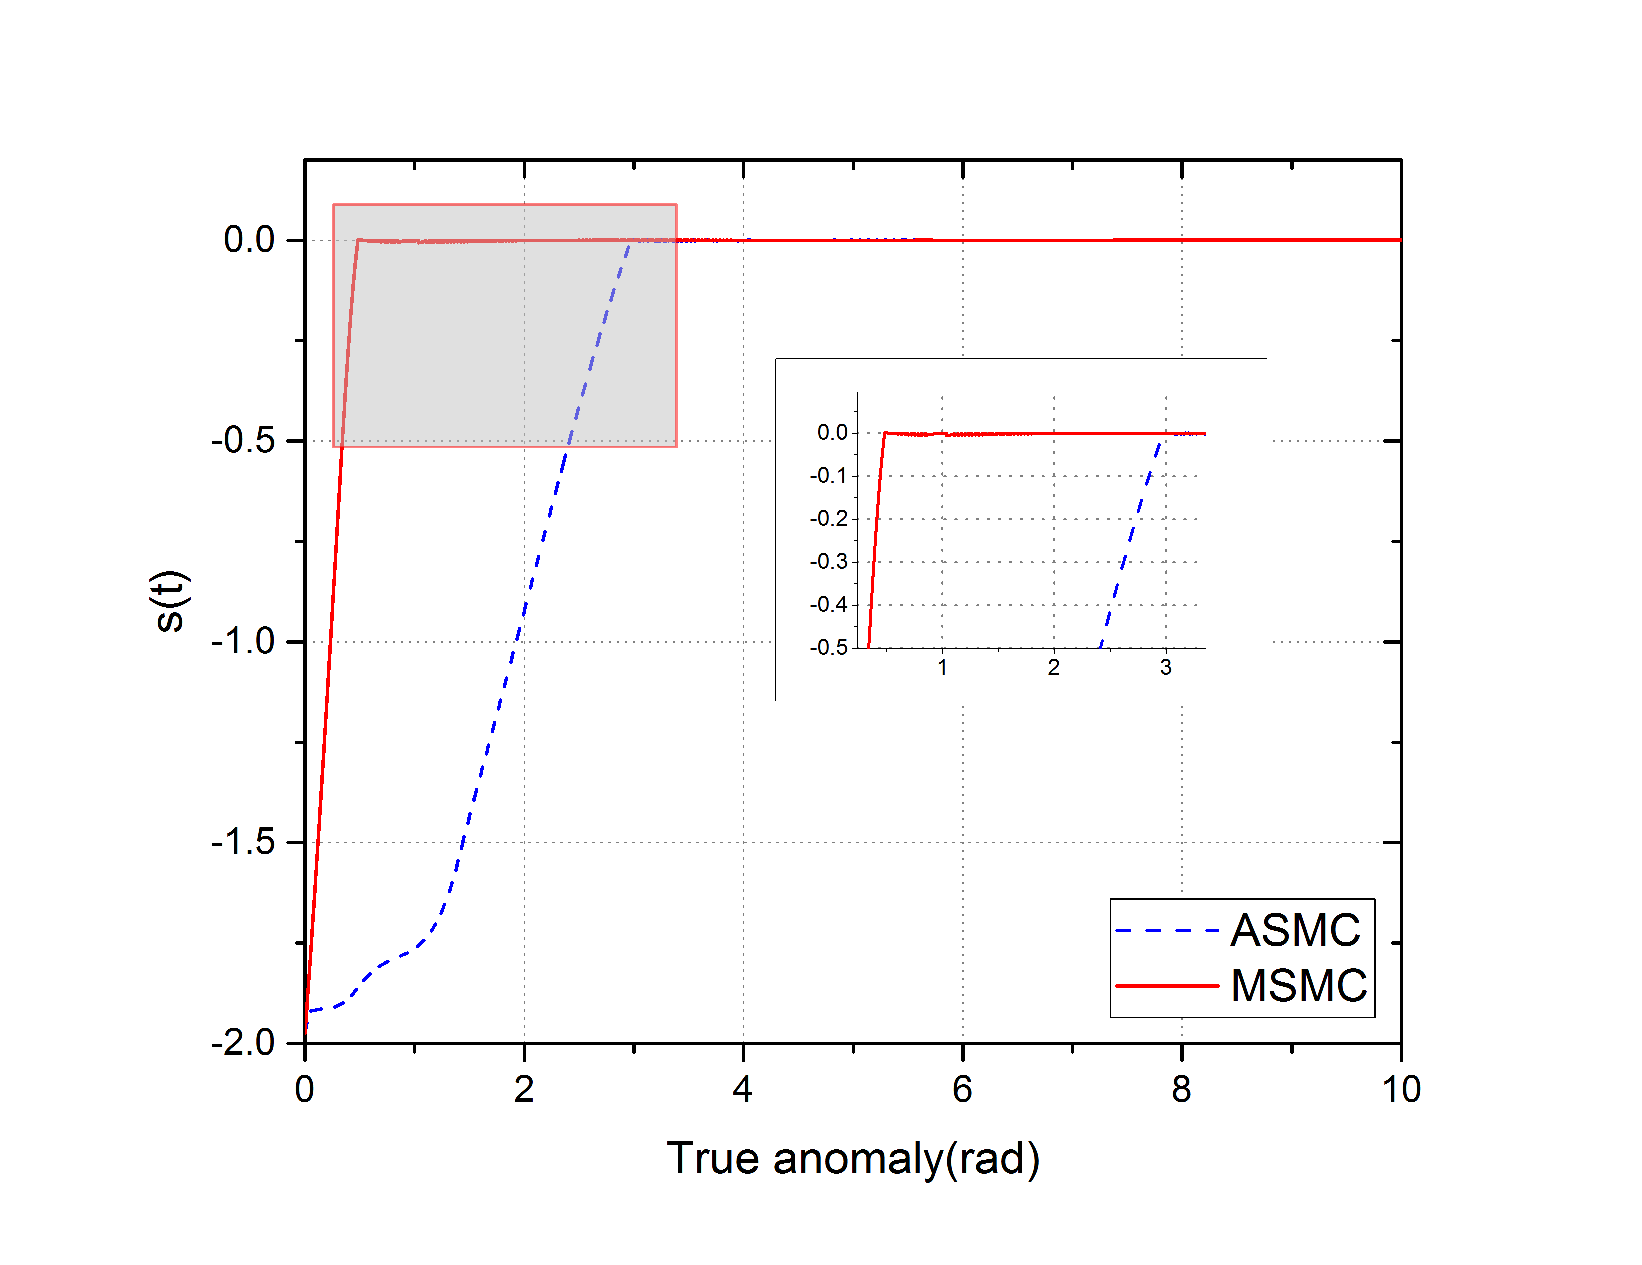
\includegraphics[width=10cm,height=7cm]{deployment_s(t).eps}
\caption{Sliding mode guidance in deployment}
\label{fig:switch}
\end{figure}

\begin{figure}
\centering
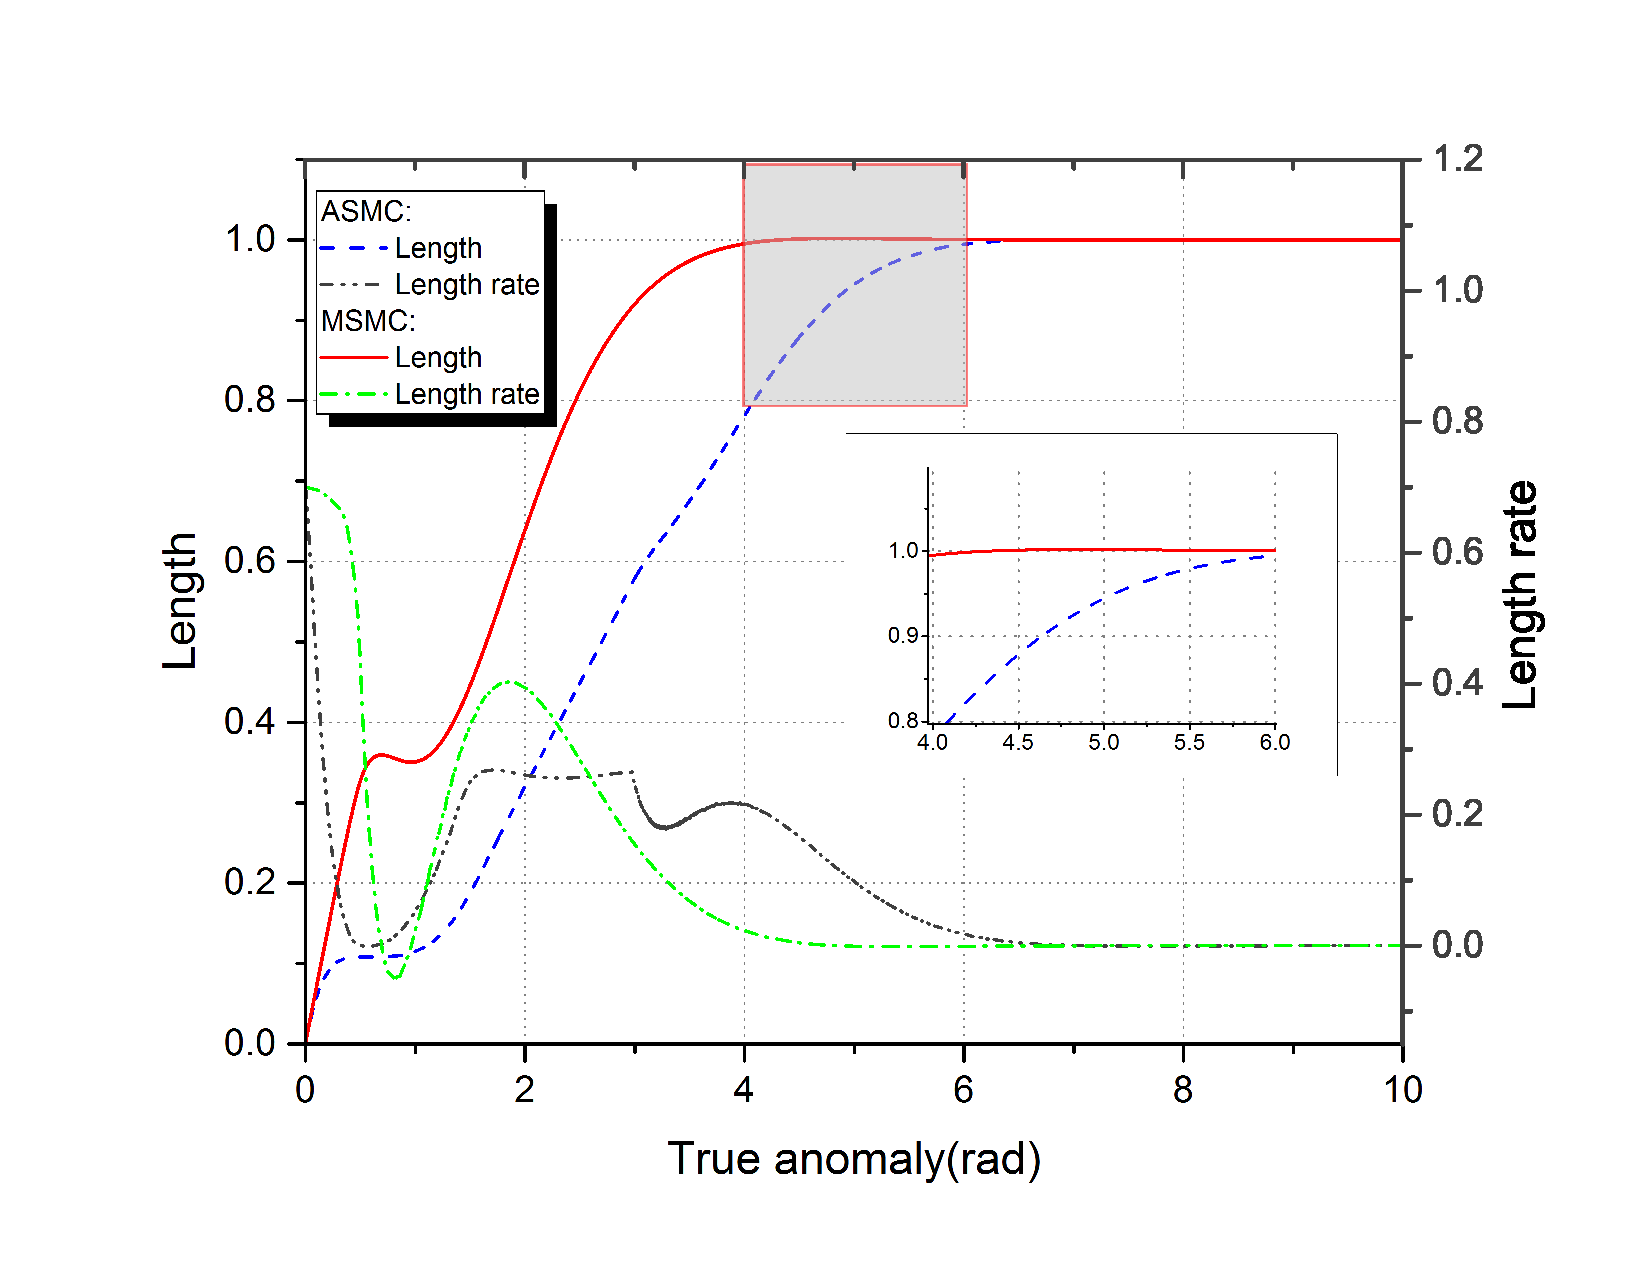
\includegraphics[width=10cm,height=7cm]{deployment_length_and_rate.eps}
\caption{Tether length / length rate state in deployment}
\label{fig:length}
\end{figure}
\begin{figure}
\centering
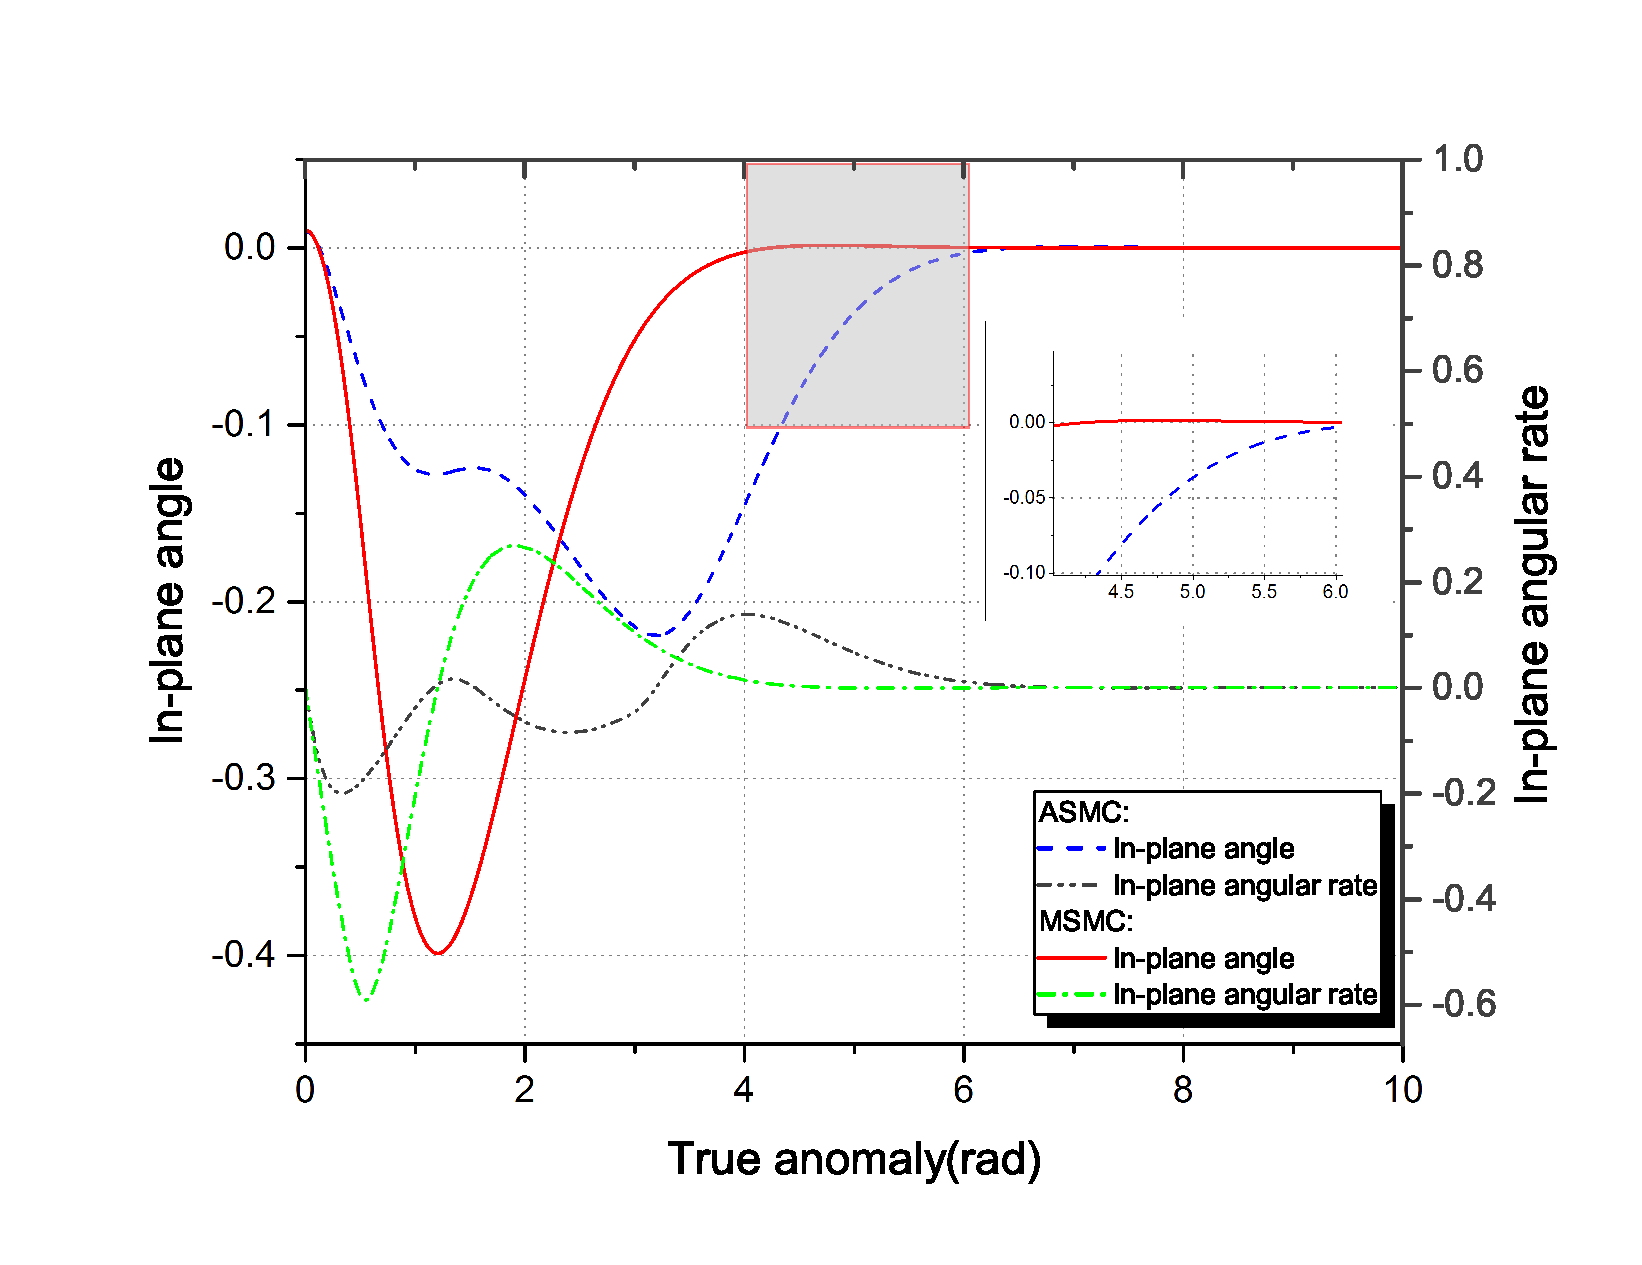
\includegraphics[width=10cm,height=7cm]{deployment_angle_and_rate.eps}
\caption{In-plane angle / angular rate state in deployment}
\label{fig:theta}
\end{figure}

\begin{figure}
\centering
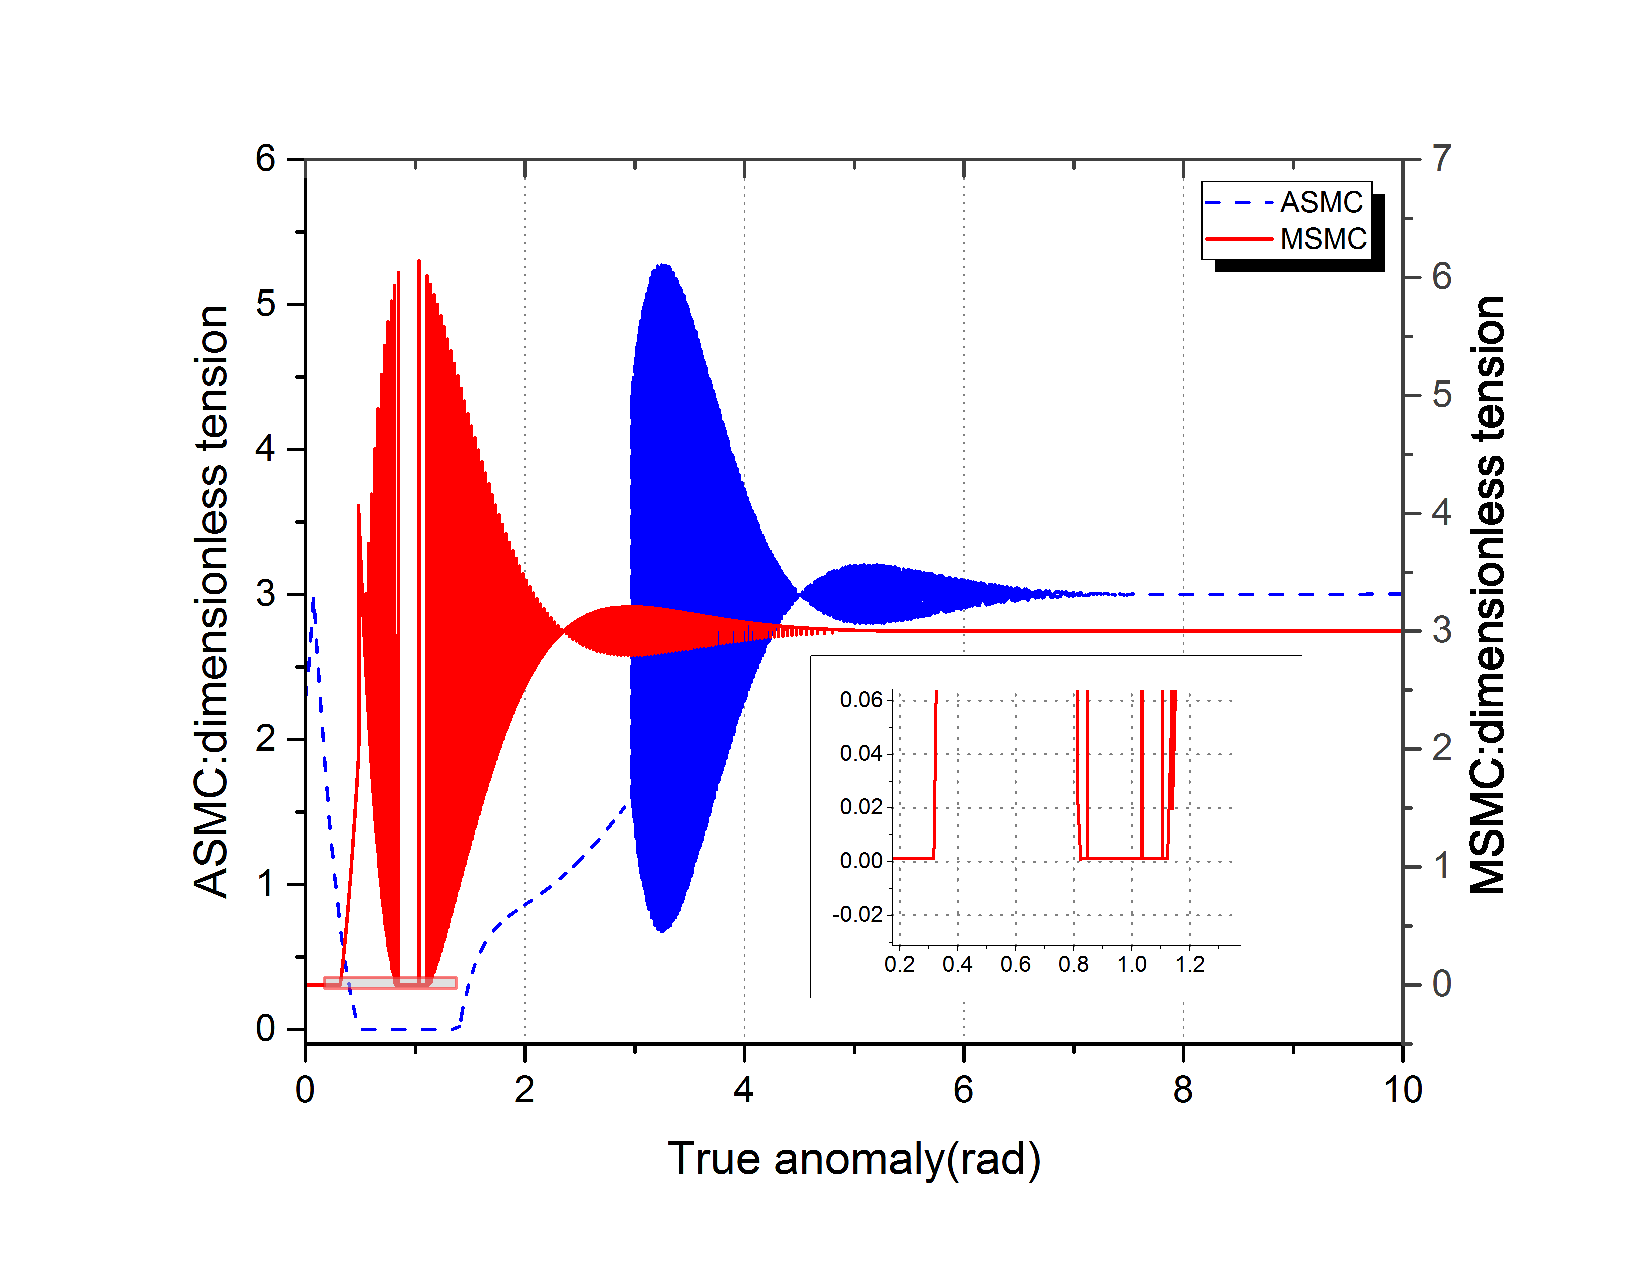
\includegraphics[width=10cm,height=7cm]{deployment_tension.eps}
\caption{Bounded tension in deployment}
\label{fig:tension}
\end{figure}
Figure \ref{fig:length} shows the length of the tether state and the rate of the length in the deployment mission. The results show that the control system MSMC and ASMC can both regulate the tether length in the deployment. In the figure, the length and the length rate are regulated to the desired states $1$ and $0$, respectively, and in addition, the length rates of two schemes fluctuate in the range $[-0.1,0.7]$ approximately which is reasonable. From this it can be seen that the deployment finishes completely at approximately 4.3 rad by using the MSMC scheme, whereas the long convergent time of the ASMC scheme for reaching the desired sliding mode surfcae results in a slow response. The trajectories of in-plane libration angles are shown in Figure \ref{fig:theta}, and the in-plane angle is variable during the spans of the libration whose variation range is $[-0.248,0.01]$ in ASMC and $[-0.4,0.01]$ in MSMC approximately . \textcolor{red}{ The rates of in-plane angle are also plotted in Fig \ref{fig:theta}, and the trajectories of the angular rates in MSMC and ASMC fluctuate in the range $[-0.7,0.3]$ approximately. In the final stage of the deployment, the angular rate states are adjusted to be zero as desired. At this point, the deployment dynamics with the ASMC and MSMC controlled have been illustrated, and from the analysis of the simulation results, the MSMC scheme performs better than ASMC in regard of the fast deployment. Furthermore, a fast deployment is usually accompanied with a large libration angle, i.e., in the YES2 phase 1 deployment, the deployment mission finishes at 4.3 rad with the maximum libration angle 48 degrees approximately\cite{williams2008deployment}, and referencing to the above mentioned results, the tethered system controlled by the MSMC scheme owns the similar performance with the fast deployment shown in the YES2 phase 1 deployment.}\par
Figure \ref{fig:tension} represents the dimensionless tension acting on the tether, and the results illustrate that the limitation occurs during the deployment mission, i.e., for the deployment with the MSMC scheme, the limitation appears at approximately 0.8 rad. Combining the bounded tension and Figure \ref{fig:switch}, once $S$ locates in the neighbourhood of the desired sliding mode surface, the tension switches in high frequency in a period time subsequently. In the end of deployment, the dimensionless tension maintains in the neighbour region of $3$, which means that the system has been stable completely, and equivalently, the input $u$ acting on the system is approximate to zero in the final. The usefulness and effectiveness of the proposed control schemes can be verified by synthesizing the above mentioned results and analysis.\par
\section{Conclusion}\label{sec:Conclusion}
A state feedback sliding mode scheme has been presented for the deployment of tethered satellites. This scheme is determined with considering input limitation and uncertain exogenous disturbance for the physical fact of the tether tension control. Theoretical analysis is exhibited to ensure that the system state converges to the desired sliding mode surface in finite time and holds in the desired sliding mode surface. The simulation results show that the deployment mission with the control scheme is effective, in which the tether length as well as the in-plane angle are not oscillatory and stay their steady state value, and furthermore, the angle excursion is reasonable and the tension meets the constraint.
\section{Acknowledgment}
This work is partially supported by the National Natural Science Foundation of China (No. 61104112, 61503097).
\section{References}
\bibliography{refdatabase}
\bibliographystyle{elsarticle-num}
\end{document}
